% filepath: d:\GitHub\DoutoradoCefet\InteligenciaComputacional\pertinecia\relatorio\relatorio_pertinencia.tex
\documentclass[a4paper,12pt]{article}

\usepackage[utf8]{inputenc}
\usepackage{amsmath}
\usepackage{graphicx}
\usepackage{float}
\usepackage{hyperref}

\title{Relatório sobre Funções de Pertinência}
\author{Doutorado CEFET}
\date{\today}

\begin{document}

\maketitle

\section{Introdução}
Este relatório apresenta as funções de pertinência implementadas no notebook \texttt{pertinencia.ipynb}. As funções de pertinência são amplamente utilizadas em lógica fuzzy para representar graus de pertencimento de elementos a conjuntos fuzzy.

\section{Funções de Pertinência}
A seguir, descrevemos as funções de pertinência implementadas:

\subsection{Função Triangular}
A função triangular é definida por três parâmetros $(a, b, c)$, onde:
\begin{itemize}
    \item $a$ é o ponto inicial onde a pertinência começa a aumentar;
    \item $b$ é o ponto onde a pertinência atinge o valor máximo (1);
    \item $c$ é o ponto final onde a pertinência retorna a 0.
\end{itemize}
A fórmula é dada por:
\[
\mu(x) =
\begin{cases}
\frac{x - a}{b - a}, & \text{se } a \leq x < b, \\
\frac{c - x}{c - b}, & \text{se } b \leq x < c, \\
0, & \text{caso contrário.}
\end{cases}
\]
Esta função é útil para modelar transições lineares simples.
\begin{figure}[H]
    \centering
    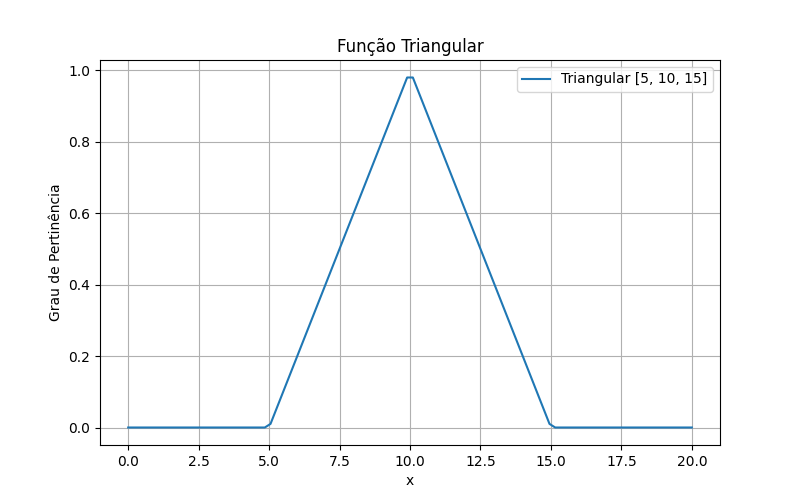
\includegraphics[width=0.8\textwidth]{img/triangular.png}
    \caption{Exemplo de função triangular com $a=5$, $b=10$, $c=15$.}
\end{figure}

\subsection{Função Trapezoidal}
A função trapezoidal é definida por quatro parâmetros $(a, b, c, d)$, onde:
\begin{itemize}
    \item $a$ e $d$ são os pontos onde a pertinência é 0;
    \item $b$ e $c$ definem a região onde a pertinência é 1.
\end{itemize}
A fórmula é:
\[
\mu(x) =
\begin{cases}
\frac{x - a}{b - a}, & \text{se } a \leq x < b, \\
1, & \text{se } b \leq x \leq c, \\
\frac{d - x}{d - c}, & \text{se } c < x \leq d, \\
0, & \text{caso contrário.}
\end{cases}
\]
Esta função é ideal para modelar transições suaves com uma região plana.
\begin{figure}[H]
    \centering
    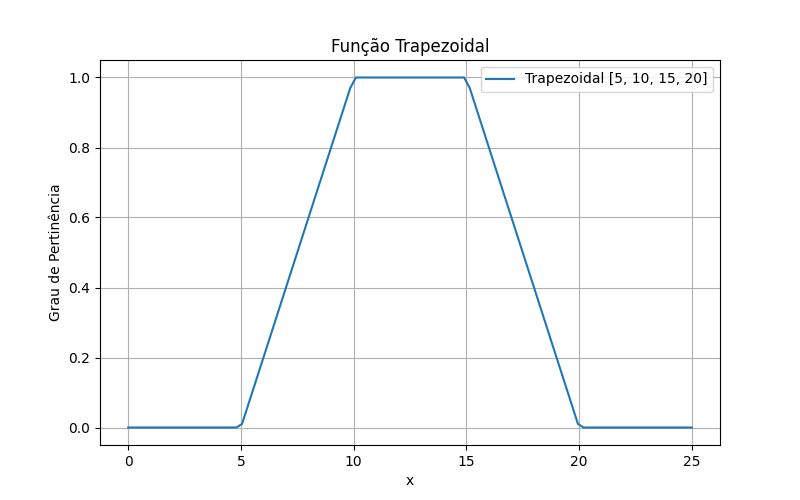
\includegraphics[width=0.8\textwidth]{img/trapezoidal.png}
    \caption{Exemplo de função trapezoidal com $a=5$, $b=10$, $c=15$, $d=20$.}
\end{figure}

\subsection{Função Gaussiana}
A função gaussiana é definida por dois parâmetros $(c, \sigma)$, onde:
\begin{itemize}
    \item $c$ é o centro da curva, onde a pertinência é máxima (1);
    \item $\sigma$ controla a largura da curva.
\end{itemize}
A fórmula é:
\[
\mu(x) = e^{-\frac{1}{2} \left( \frac{x - c}{\sigma} \right)^2}.
\]
Esta função é amplamente utilizada devido à sua suavidade e simetria.
\begin{figure}[H]
    \centering
    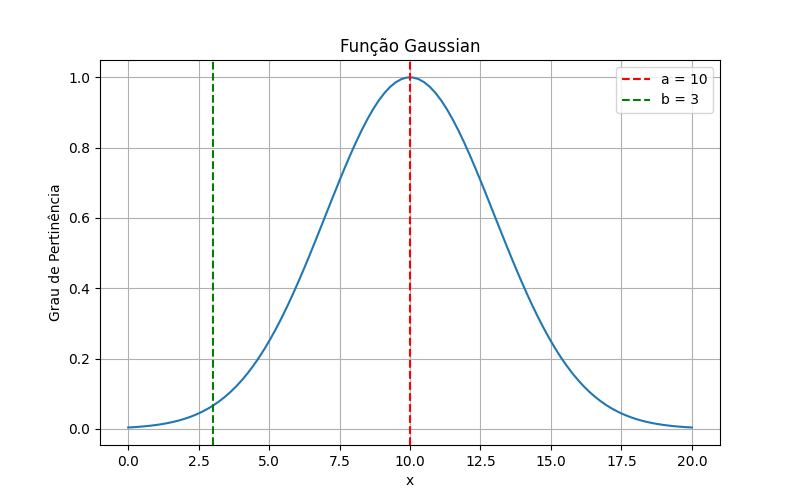
\includegraphics[width=0.8\textwidth]{img/gaussian.png}
    \caption{Exemplo de função gaussiana com $c=10$, $\sigma=3$.}
\end{figure}

\subsection{Função Sigmoidal}
A função sigmoidal é definida por dois parâmetros $(a, c)$, onde:
\begin{itemize}
    \item $a$ controla a inclinação da curva;
    \item $c$ é o ponto central onde a pertinência é 0.5.
\end{itemize}
A fórmula é:
\[
\mu(x) = \frac{1}{1 + e^{-a(x - c)}}.
\]
Esta função é útil para modelar transições suaves e contínuas.
\begin{figure}[H]
    \centering
    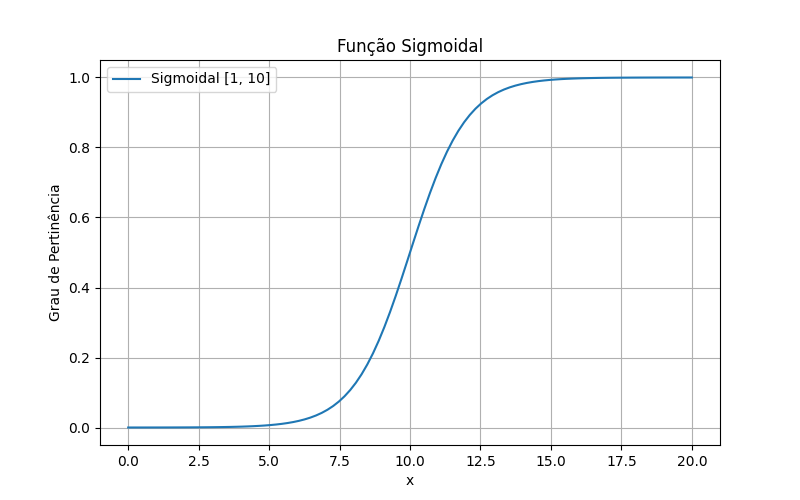
\includegraphics[width=0.8\textwidth]{img/sigmoidal.png}
    \caption{Exemplo de função sigmoidal com $a=1$, $c=10$.}
\end{figure}

\subsection{Função Z}
A função Z é definida por dois parâmetros $(a, b)$, onde:
\begin{itemize}
    \item $a$ é o ponto onde a pertinência começa a diminuir;
    \item $b$ é o ponto onde a pertinência atinge 0.
\end{itemize}
A fórmula é:
\[
\mu(x) =
\begin{cases}
1, & \text{se } x \leq a, \\
1 - 2\left(\frac{x - a}{b - a}\right)^2, & \text{se } a < x < b, \\
0, & \text{se } x \geq b.
\end{cases}
\]
Esta função é usada para modelar transições decrescentes suaves.
\begin{figure}[H]
    \centering
    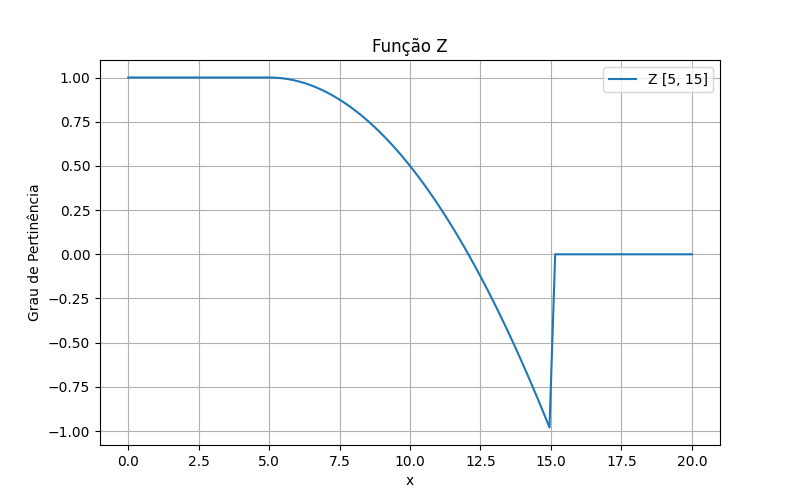
\includegraphics[width=0.8\textwidth]{img/z.png}
    \caption{Exemplo de função Z com $a=5$, $b=15$.}
\end{figure}

\subsection{Função S}
A função S é definida por dois parâmetros $(a, b)$, onde:
\begin{itemize}
    \item $a$ é o ponto onde a pertinência começa a aumentar;
    \item $b$ é o ponto onde a pertinência atinge 1.
\end{itemize}
A fórmula é:
\[
\mu(x) =
\begin{cases}
0, & \text{se } x \leq a, \\
2\left(\frac{x - a}{b - a}\right)^2, & \text{se } a < x < b, \\
1, & \text{se } x \geq b.
\end{cases}
\]
Esta função é usada para modelar transições crescentes suaves.
\begin{figure}[H]
    \centering
    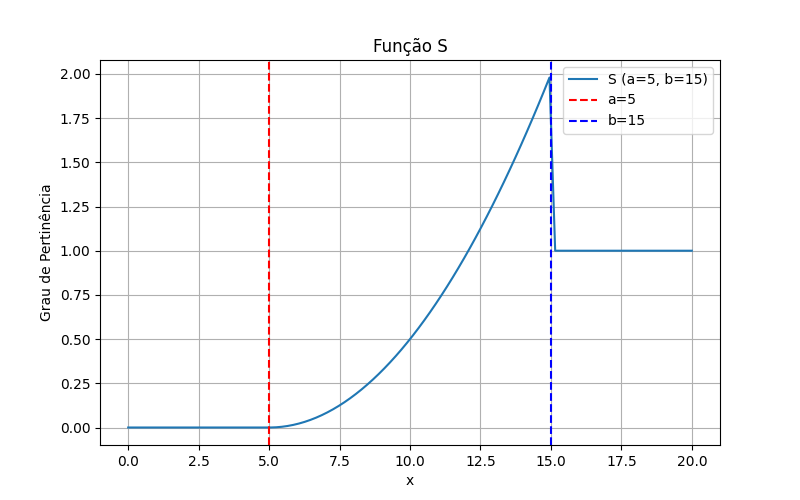
\includegraphics[width=0.8\textwidth]{img/s.png}
    \caption{Exemplo de função S com $a=5$, $b=15$.}
\end{figure}

\subsection{Função Pi}
A função Pi combina as funções S e Z, sendo definida por três parâmetros $(a, b, c)$:
\begin{itemize}
    \item $a$ e $c$ definem os pontos de transição inicial e final;
    \item $b$ é o ponto central onde a pertinência é máxima.
\end{itemize}
A fórmula é:
\[
\mu(x) =
\begin{cases}
\text{S}(x, a, b), & \text{se } x < b, \\
\text{Z}(x, b, c), & \text{se } x \geq b.
\end{cases}
\]
Esta função é útil para modelar transições suaves em ambos os lados.
\begin{figure}[H]
    \centering
    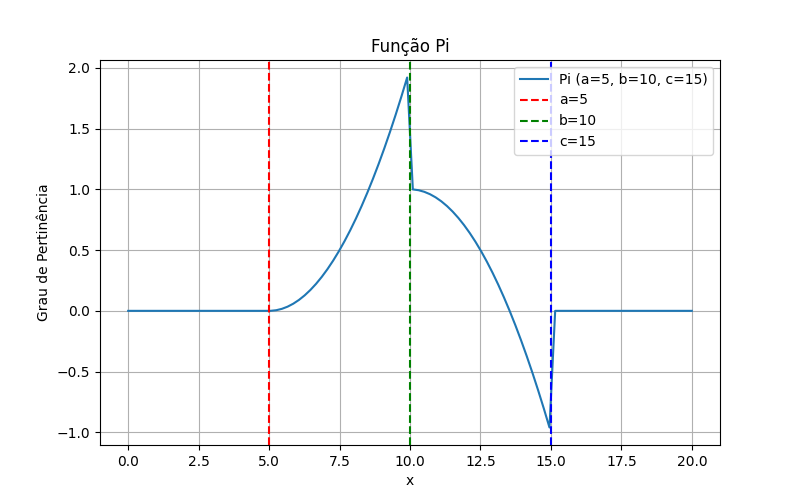
\includegraphics[width=0.8\textwidth]{img/pi.png}
    \caption{Exemplo de função Pi com $a=5$, $b=10$, $c=15$.}
\end{figure}

\subsection{Função Bell}
A função Bell é definida por três parâmetros $(a, b, c)$, onde:
\begin{itemize}
    \item $a$ controla a largura da curva;
    \item $b$ controla a inclinação;
    \item $c$ é o centro da curva.
\end{itemize}
A fórmula é:
\[
\mu(x) = \frac{1}{1 + \left|\frac{x - c}{a}\right|^{2b}}.
\]
Esta função é usada para modelar curvas suaves e simétricas.
\begin{figure}[H]
    \centering
    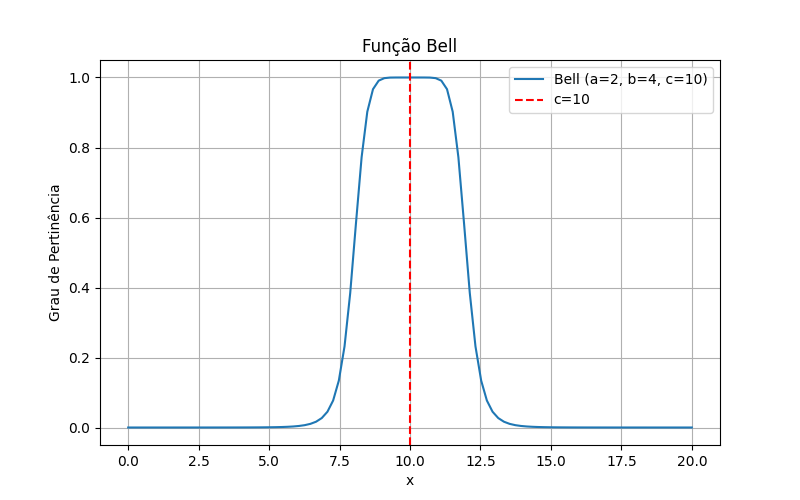
\includegraphics[width=0.8\textwidth]{img/bell.png}
    \caption{Exemplo de função Bell com $a=2$, $b=4$, $c=10$.}
\end{figure}

\subsection{Função Singleton}
A função Singleton é definida por um parâmetro $c$, onde:
\begin{itemize}
    \item $c$ é o ponto onde a pertinência é 1.
\end{itemize}
A fórmula é:
\[
\mu(x) =
\begin{cases}
1, & \text{se } x = c, \\
0, & \text{caso contrário.}
\end{cases}
\]
Esta função é usada para representar valores exatos.
\begin{figure}[H]
    \centering
    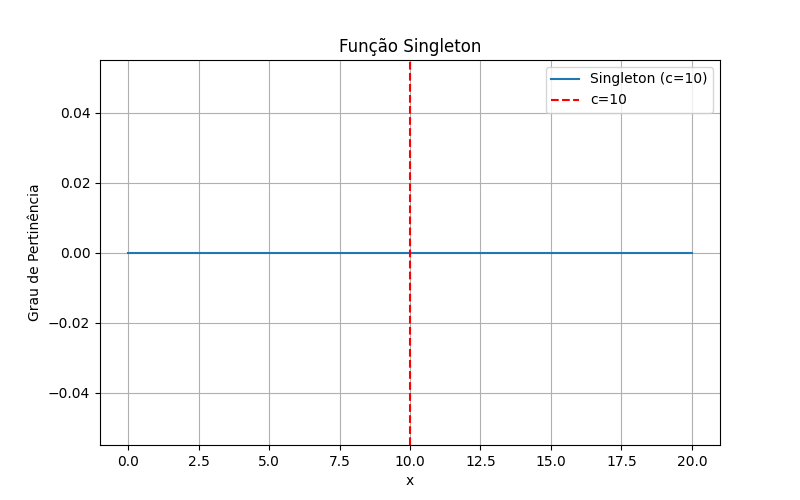
\includegraphics[width=0.8\textwidth]{img/singleton.png}
    \caption{Exemplo de função Singleton com $c=10$.}
\end{figure}

\subsection{Função Linear}
A função Linear é definida por dois parâmetros $(a, b)$, onde:
\begin{itemize}
    \item $a$ é o ponto onde a pertinência começa a aumentar;
    \item $b$ é o ponto onde a pertinência atinge 1.
\end{itemize}
A fórmula é:
\[
\mu(x) =
\begin{cases}
0, & \text{se } x \leq a, \\
\frac{x - a}{b - a}, & \text{se } a < x < b, \\
1, & \text{se } x \geq b.
\end{cases}
\]
Esta função é útil para modelar transições lineares crescentes.
\begin{figure}[H]
    \centering
    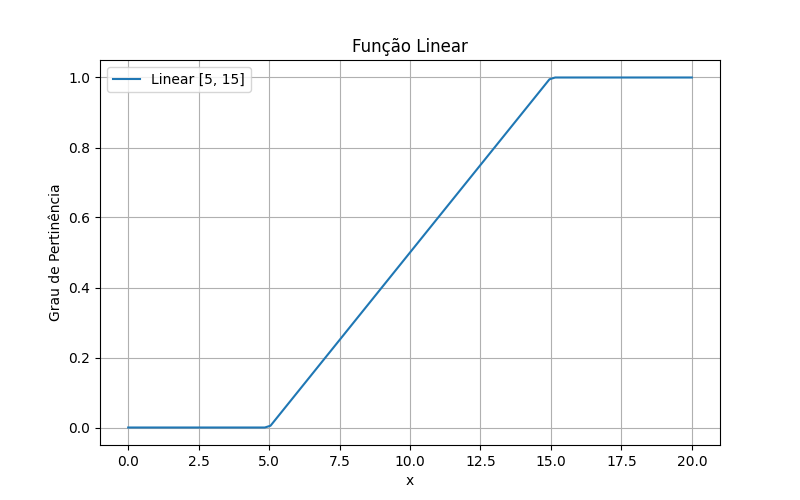
\includegraphics[width=0.8\textwidth]{img/linear.png}
    \caption{Exemplo de função Linear com $a=5$, $b=15$.}
\end{figure}

\section{Conclusão}
As funções de pertinência descritas neste relatório são ferramentas fundamentais para modelagem em lógica fuzzy. Cada função possui características específicas que as tornam adequadas para diferentes aplicações.

\end{document}